
\documentclass[11pt]{article}
\usepackage[english]{babel}
\usepackage[utf8]{inputenc}
\usepackage{amsmath}
\usepackage{mathtools}
\usepackage{amssymb}
\usepackage{amsthm}
\usepackage{color}
\usepackage[margin=1in,nohead]{geometry}
\usepackage[mathscr]{euscript}
\usepackage{enumitem}
\usepackage{url}
\usepackage{listings}
\usepackage{caption}
\usepackage{subcaption}
\usepackage{hyperref}

\newcommand{\mc}{\mathcal}
\newcommand{\mbf}{\mathbf}
\newcommand{\mb}{\mathbb}
\newcommand{\msc}{\mathscr}
\newcommand{\goesto}{\rightarrow}
\newcommand{\note}{{\bf Note: }}
\newcommand{\vspan}{\text{span}}

\newcommand{\R}{\mb{R}}
\newcommand{\nat}{\mb{N}}

\newcommand{\A}{\mathbf{A}}
\newcommand{\B}{\mathbf{B}}
\newcommand{\C}{\mathbf{C}}
\newcommand{\X}{\mathbf{X}}
\newcommand{\x}{\mathbf{x}}
\newcommand{\y}{\mathbf{y}}
\newcommand{\z}{\mathbf{z}}
\renewcommand{\b}{\mathbf{b}}
\renewcommand{\u}{\mathbf{u}}
\renewcommand{\v}{\mathbf{v}}
\newcommand{\ones}{\mathbf{1}}
\newcommand{\zero}{\mathbf{0}}

\newcommand{\Eqn}[1]{\begin{align*} #1 \end{align*}}
\newcommand{\bbm}{\begin{bmatrix}}
\newcommand{\ebm}{\end{bmatrix}}
\newcommand{\bpm}{\begin{pmatrix}}
\newcommand{\epm}{\end{pmatrix}}

\newcommand{\Sol}{\par {\bf Solution:}}
\newcommand{\sample}[1]{#1_1 , \dots , #1_n}
\newcommand{\order}[1]{X_{(#1)}}
\newcommand{\Partial}[1]{\frac{\partial}{\partial #1}}

\DeclareMathOperator*{\argmin}{\arg\min}
\DeclareMathOperator*{\argmax}{\arg\max}

\setlength{\parskip}{6pt}
\setlength{\parindent}{0pt}
\allowdisplaybreaks[4]
\lstset{
  basicstyle=\ttfamily,
  columns=fullflexible,
  frame=single,
  breaklines=true,
  postbreak=\mbox{\textcolor{red}{$\hookrightarrow$}\space},
}

\begin{document}

\begin{center}
\Large{
\textbf{STP 502, Spring 2023, Homework 4} \\
Due: Monday, Feb 20, 2023. \\
Shu Wan (1226038322)
}
\end{center}

\subsection*{7.12}

Let $\sample{X}$ be a random sample from a population with pmf

\[
P_\theta(X = x) = \theta^x(1-\theta)^{1-x}, \quad x = 0 \text{ or } 1, \quad 0 \le \theta \le \frac{1}{2}.
\]
\begin{enumerate}[label=(\alph*)]
    \item Find the method of moments estimator and MLE of $\theta$.
    \item Find the mean squared errors of each of the estimators.
\end{enumerate}

\Sol
\begin{enumerate}[label=(\alph*)]
    \item \textbf{Method of moments} \\
    $X \sim \text{Bernoulli}(\theta)$
        \[
        EX = \theta = \sum X_i / n = \bar X \Rightarrow \Tilde{\theta} = \bar X
        \]
    \textbf{MLE} \\
    From Example 7.2.7, we know that the MLE estimator for Bernoulli($\theta$) is $\bar X$ if $\theta \in [0, 1]$. However, in this case, $\theta$ is restricted in $[0, 1/2]$. The likelihood function $L$ is monotone increasing in $[0, \bar X]$ Hence, the  MLE estimator for this restricted case is $\hat \theta = \max \{\bar X, 1/2\}$.
    
    \item 
    \textbf{Method of moments} \\
    \[
    \text{MSE}(\Tilde{\theta}) = \text{Var}(\Tilde{\theta}) + \text{bias}(\Tilde{\theta}) = \text{Var}(\Tilde{\theta}) = \frac{\theta(1 - \theta)}{n}
    \]

    \textbf{MLE} \\
    \[
    \text{MSE}(\hat \theta) = \begin{cases}
    \frac{\theta(1 - \theta)}{n} & \text{if } \bar X \le 1/2, \\
    (1/2- \theta)^2 {n \choose \sum x_i} (\theta)^{\sum x_i}(1-\theta)^{n-\sum x_i} & \text{if } \bar X > 1/2.
    \end{cases}
    \]
    
    \textbf{Note} The MLE works on restricted parameter space, however I'm not sure how does it apply to method of moments estimators. Some suggests to treat restricted parameter space as a constrained optimization problem along with method of moments estimator.
\end{enumerate}

\subsection*{7.13}
Let $\sample{X}$ be a sample from a population with double exponential pdf
\[
f(x|\theta) = \frac{1}{2}e^{-|x-\theta|}, \quad -\infty < x < \infty, \quad -\infty < \theta < \infty.
\]

Find the MLE of $\theta$. ( Hint : Consider the case of even $n$ separate from that of odd $n$, and find the MLE in terms of the order statistics. A complete treatment of this problem is given in Norton 1984.)

\Sol

The log-likelihood function 
\[
l = \log L(\theta) = -n\log 2 - \sum |x_i - \theta|
\]
The maximum of $l$ is achieved when $\Psi = \sum |x_i - \theta|$ is minimal.

The absolute difference function $\Psi$ is continuous everywhere but non-differentiable when $\theta = x_i, \forall i$.

When exists, the derivative of $\Psi$ is 
\[
\frac{d}{d\theta}\Psi(\theta) = (\sum (x_i - \theta)^{1/2})^{'} = \sum \text{sign}(x_i - \theta).
\]
Without loss of generality, we assume $X_i$ is sorted form the smallest to the largest. The value of $\Psi$ is
\[
\Psi(\theta) = \begin{cases}
    n & \theta < x_1 \\
    n - 2\times j & x_j < \theta < x_{j+1} \\
    -n & \theta > x_n
\end{cases}
\]

When $n$ is even, the $\Psi^{'}(\theta)$ is zero, and hence any value in $(x_{n/2}, x_{n/2+1})$ is a MLE for $\theta$. We can pick the mid-point $\hat{\theta} = 1/2(x_{n/2} + x_{n/2+1})$ as the MLE.

When $n$ is odd, the derivative $\Psi(\theta)$ never equals to 0. In this case, it's easy to see that $\Psi(\theta)$ is decreasing in $(-\infty, x_{(n+1)/2}]$ and increasing in $[x_{(n+1)/2}, \infty)$. Hence, $\hat \theta = x_{(n+1)/2}$ is the minimum for $\Psi$.

Thus the sample median is a MLE for $\theta$.

To illustrate this, we plot $\Psi(\theta)$ and $\Psi^{'}(\theta)$ in Fig. (\ref{fig:four graphs}). Code for generating the plots are in Code. (\ref{Code1}).

\lstinputlisting[language=R, caption={R Code}, label=Code1]{hw4.R}

\begin{figure}[h]
     \centering
     \begin{subfigure}[b]{0.48\textwidth}
         \centering
         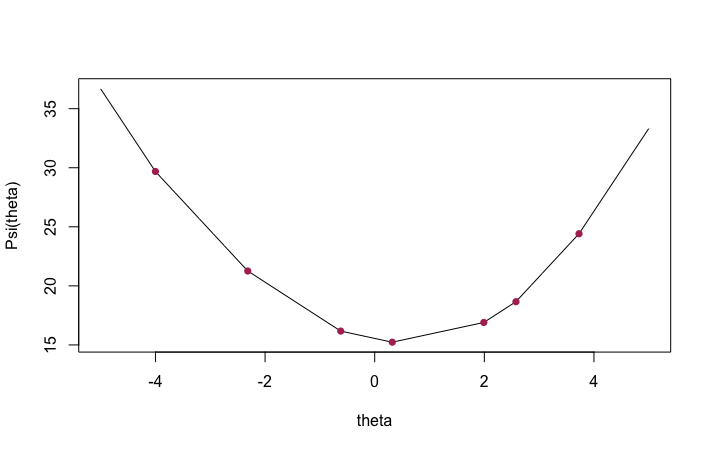
\includegraphics[width=\textwidth]{fig/hw4-1.png}
         \caption{$\Psi(\theta), n = 7$}

     \end{subfigure}
     \hfill
     \begin{subfigure}[b]{0.48\textwidth}
         \centering
         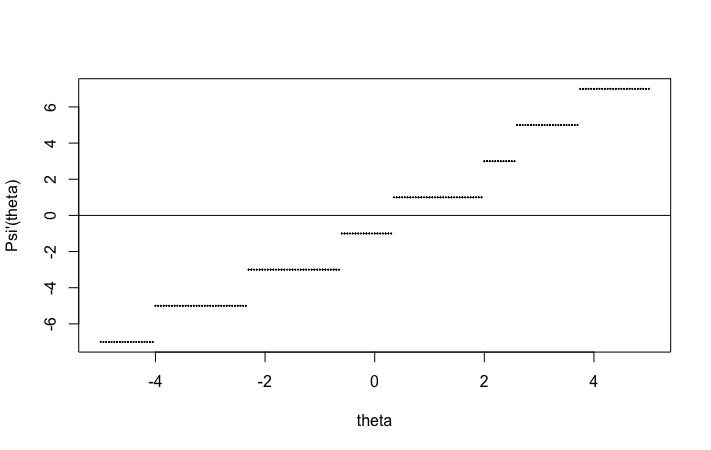
\includegraphics[width=\textwidth]{fig/hw4-2.png}
         \caption{$\Psi^{'}(\theta), n = 7$}

     \end{subfigure}
          \begin{subfigure}[b]{0.48\textwidth}
         \centering
         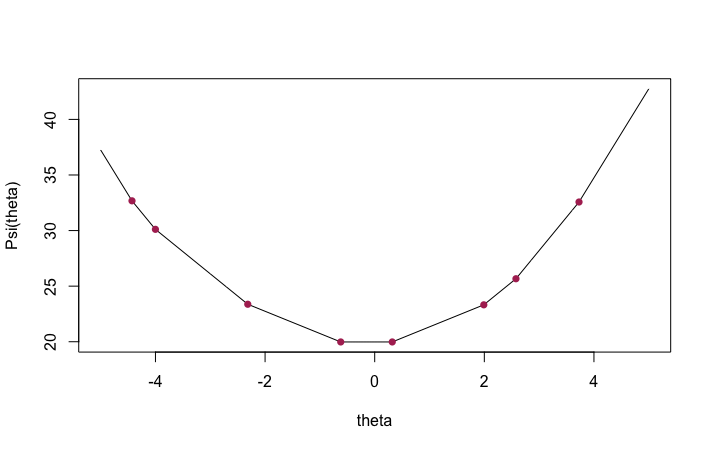
\includegraphics[width=\textwidth]{fig/hw4-3.png}
         \caption{$\Psi(\theta), n = 8$}

     \end{subfigure}
     \hfill
     \begin{subfigure}[b]{0.48\textwidth}
         \centering
         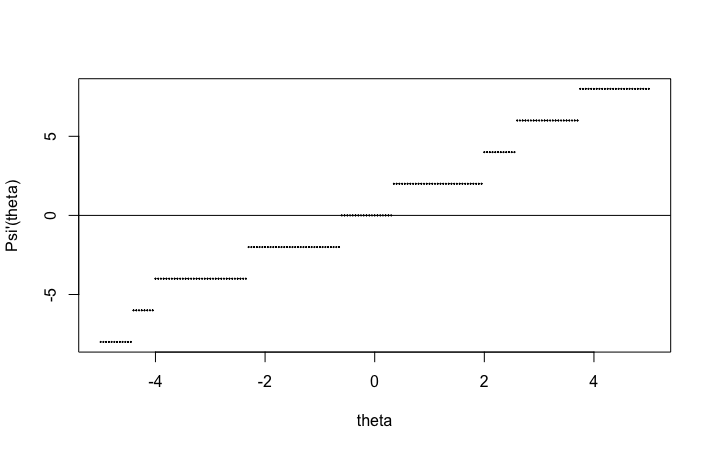
\includegraphics[width=\textwidth]{fig/hw4-4.png}
         \caption{$\Psi^{'}(\theta), n = 8$}

     \end{subfigure}
     \caption{$\Psi$ when $n$ is odd and even.}
    \label{fig:four graphs}
\end{figure}

\subsection*{7.22}
This exercise will prove the assertions in Example 7.2.16, and more. Let $\sample{X}$ be: a random sample from a $n(\theta, \sigma^2)$ population, and suppose that the prior distribution on $\theta$ is $n(\mu, \tau^2)$. Here we assume that $\sigma^2$, $\mu$, and $\tau^2$ are all known.

\begin{enumerate}[label=(\alph*)]
    \item Find the joint pdf of $\bar X$ and $\theta$.
    \item Show that $m(\bar x| \sigma^2, \mu, \tau^2)$, the marginal distribution of $\bar X$, is $n(\mu, (\sigma^2/n) + \tau^2)$.
    \item Show that $\pi(\theta|\bar x, \sigma^2, \mu, \tau^2)$, the posterior distribution of $\theta$, is normal with mean and variance given by (7.2.10).
\end{enumerate}

\Sol
\begin{enumerate}[label=(\alph*)]
    \item
    \[
    f(\bar X, \theta) = f(\bar X | \theta) \cdot \pi(\theta) = N(\theta, \sigma^2/n) \cdot N(\mu, \tau^2) = \frac{\sqrt{n}}{\sqrt{2\pi}\sigma}e^{-n(\bar x - \theta)^2/2\sigma^2} \cdot \frac{1}{\sqrt{2\pi}\mu}e^{-(\theta - \mu)^2/2\tau^2}.
    \]
    
    \item
    We can also factorize the joint distribution as
    \[
    f(\bar X, \theta) = \pi(\theta|\bar X) m(\bar X).
    \]
    If so, we have the solutions for part(b) and (c).
    To simplify notation, let $\alpha^2 = \sigma^2/n$
    \begin{align*}
        f(\bar X, \theta) &= \frac{1}{2\pi \alpha \tau}\exp \Bigl\{-\frac{1}{2} \Bigl( \frac{\bigl(\bar X - \theta)^2}{\alpha^2} + \frac{(\theta - \mu)^2}{\tau^2} \Bigr) \Bigr\} \\
        &= \frac{1}{2\pi \alpha \tau} \exp \Bigl\{-\frac{\tau^2 + \alpha^2}{2\alpha^2\tau^2} \Bigl( \theta^2 - 2\frac{\tau^2\bar X + \alpha^2\mu}{\tau^2 + \alpha^2}\theta + \frac{\tau^2\bar X^2 + \alpha^2\mu^2}{\tau^2 + \alpha^2} \Bigr) \Bigr\} \\
        &= \frac{1}{2\pi \alpha \tau} \cdot 
        \exp \Bigl\{-\frac{\tau^2 + \alpha^2}{2\alpha^2\tau^2} \Bigl( \theta - \frac{\tau^2\bar X + \alpha^2\mu}{\tau^2 + \alpha^2} \Bigr)^2 \Bigr\} \cdot 
        \exp \Bigl\{-\frac{\tau^2 + \alpha^2}{2\alpha^2\tau^2} \Bigl( \frac{\tau^2\bar X^2 + \alpha^2\mu^2}{\tau^2 + \alpha^2} -  (\frac{\tau^2\bar X + \alpha^2\mu}{\tau^2 + \alpha^2})^2 \Bigr) \Bigr\} \\
        &= \frac{1}{2\pi \alpha \tau} \cdot 
        \exp \Bigl\{-\frac{\tau^2 + \alpha^2}{2\alpha^2\tau^2} \Bigl( \theta - \frac{\tau^2\bar X + \alpha^2\mu}{\tau^2 + \alpha^2} \Bigr)^2 \Bigr\} \cdot 
        \exp \Bigl\{ -\frac{1}{2}\cdot \frac{(\bar X - \mu)^2}{\tau^2 + \alpha^2} \Bigr\} \\
        &= \frac{1}{\sqrt{2\pi} \sqrt{\frac{\alpha^2 \tau^2}{\tau^2 + \alpha^2}}} \cdot 
        \exp \Bigl\{-\frac{1}{2} \cdot \frac{( \theta - \frac{\tau^2\bar X + \alpha^2\mu}{\tau^2 + \alpha^2})^2}{\frac{\alpha^2\tau^2}{\tau^2 + \alpha^2}} \Bigr\} \cdot
        \frac{1}{\sqrt{2\pi} \sqrt{\tau^2 + \alpha^2}} \cdot
        \exp \Bigl\{ -\frac{1}{2}\cdot \frac{(\bar X - \mu)^2}{\tau^2 + \alpha^2} \Bigr\} \\
        &= n_{\theta}(\frac{\tau^2\bar X + \alpha^2\mu}{\tau^2 + \alpha^2}, \frac{\alpha^2 \tau^2}{\tau^2 + \alpha^2}) \cdot n_{\bar X}(\mu, \tau^2 + \alpha^2).
    \end{align*}
    
    Hence, $m(\bar x| \sigma^2, \mu, \tau^2) \sim n(\mu, (\sigma^2/n) + \tau^2)$,
    \item
    and $\pi(\theta|\bar x, \sigma^2, \mu, \tau^2) \sim n(\frac{\tau^2\bar X + \alpha^2\mu}{\tau^2 + \alpha^2}, \frac{\alpha^2 \tau^2}{\tau^2 + \alpha^2})$, where $\alpha^2 = \sigma^2/n$.
\end{enumerate}

\subsection*{7.23}
If $S^2$ is the sample variance based on a sample of size $n$ from a normal population, we know that $(n - 1 ) S^2/\sigma^2$ has a $\chi_{n-1}^2$ distribution. The conjugate prior for $\sigma^2$ is the \emph{inverted gamma} pdf, $\text{IG}(\alpha, \beta)$ , given by
\[
\pi(\sigma^2) = \frac{1}{\Gamma(\alpha)\beta^\alpha}\frac{1}{(\sigma^2)^{\alpha + 1}}e^{-1/(\beta\alpha^2)}, \quad 0 < \sigma^2 < \infty.
\]
where $\alpha$ and $\beta$ are positive constants. Show that the posterior distribution of $\sigma^2$ is $\text{IG}(\alpha + \frac{n+1}{2}, [\frac{(n-1)S^2}{2} + \frac{1}{\beta}]^{-1})$. Find the mean of this distribution, the Bayes estimator of $\sigma^2$.

\Sol

First, let $Y = S^2$, $X = \frac{n-1}{\sigma^2}S^2 \sim \chi^2_{n-1}$, the pdf for $Y$ is
\[
f(S^2|\sigma^2) = \frac{1}{2^{n-1/2}\Gamma((n-1)/2)}(\frac{n-1}{\sigma^2}S^2)^{[(n-1)/2] - 1}e^{-(n-1)S^2/2\sigma^2} \cdot \frac{n-1}{\sigma^2}.
\]
With the prior distribution $\pi(\sigma^2)$ is given, we have
\begin{align*}
    \pi(\sigma^2|S^2) &\propto f(S^2|\sigma^2) \cdot \pi(\sigma^2) \\
    &\propto (\frac{1}{\sigma^2})^{(n-1)/2 - 1} e^{-(n-1)S^2/2\sigma^2} \frac{1}{\sigma^2} \cdot 
    \frac{1}{(\sigma^2)^{\alpha + 1}}e^{-1/\beta\sigma^2} \\
    &\propto (\frac{1}{\sigma^2})^{(n-1)/2 + \alpha + 1} e^{-(\frac{(n-1)S^2}{2} + \frac{1}{n})\frac{1}{\sigma^2}}
\end{align*}
Observing the kernel of above equation, we have
$\pi(\sigma^2|S^2) \sim \text{IG}(\alpha + \frac{n-1}{2}, [\frac{(n-1)S^2}{2} + \frac{1}{n}]^{-1}).$

The posterior mean is $E(\sigma^2|S^2) = \frac{\frac{(n-1)S^2}{2} + \frac{1}{n}}{\alpha + \frac{n-1}{2} - 1}$, and this is the Bayes estimator of $\sigma^2$.

\subsection*{7.24}

Let $\sample{X}$ be iid Poisson($\lambda$) , and let $\lambda$ have a $\text{gamma}(\alpha, \beta)$ distribution, the conjugate family for the Poisson.
\begin{enumerate}[label=(\alph*)]
    \item Find the posterior distribution of $\lambda$.
    \item Calculate the posterior mean and variance.
    
\end{enumerate}

\Sol
\begin{enumerate}[label=(\alph*)]
    \item
    Let $Y = \sum x_i$, then $Y \sim \text{Poi}(n\lambda)$.
    We have
    \begin{align*}
        \pi(\lambda|y) &\propto f(y|\lambda) \cdot \pi(\lambda) \\
        &\propto \frac{(ny)^y e^{-n\lambda}}{y!} \cdot \frac{1}{\Gamma(\alpha)\beta^\alpha}\lambda^{\alpha - 1}e^{-\lambda/\beta} \\
        &\propto \lambda^{y+\alpha - 1}e^{-(n + 1/\beta) \lambda}.
    \end{align*}
    Thus,
    \[
    \pi(\lambda|y) \sim \text{gamma}(\sum x_i + \alpha, (n+ 1/\beta)^{-1}). 
    \]
    \item
    The posterior mean is 
    \[
    E(\pi(\lambda|y)) = \frac{\sum x_i + \alpha}{n+ 1/\beta},
    \]
    and the variance is 
    \[
    \text{Var}(\pi(\lambda|y)) = \frac{\sum x_i + \alpha}{(n+ 1/\beta)^2}.
    \]
\end{enumerate}

\subsection*{7.25}
We examine a generalization of the hierarchical (Bayes) model considered in Example 7.2.16 and Exercise 7.22. Suppose that we observe $\sample{X}$, where
\begin{align*}
    X_i|\theta_i \sim n(\theta_i, \sigma^2), && i = 1, \dots, n, && \text{independent,} \\
    \theta_i \sim n(\mu, \tau^2), && i = 1, \dots, n, && \text{independent.}
\end{align*}

\begin{enumerate}[label=(\alph*)]
    \item Show that the marginal distribution of $X_i$ is $n(\mu, \sigma^2 + \tau^2)$ and that, marginally, $\sample{X}$ are iid. (Empirical Bayes analysis would use the marginal distribution
of the $X_i$s to estimate the prior parameters $\mu$ and $\tau^2$. See Miscellanea 7.5.6).
    \item Show, in general, that if
    \begin{align*}
    X_i|\theta_i \sim f(x|\theta_i), && i = 1, \dots, n, && \text{independent,} \\
    \theta_i \sim \pi(\theta|\tau), && i = 1, \dots, n, && \text{independent,}
    \end{align*}
    then marginally $\sample{X}$ are iid.
\end{enumerate}

\Sol
\begin{enumerate}[label=(\alph*)]
    \item
    From Exercise 7.22, we know that for any $X_i$, the marginal distribution of $X_i$ is 
    \[
    m(X_i) \sim n(\mu, \sigma^2 + \tau^2).
    \]
    Therefore, $\sample{X}$ are identically distributed.
    We only need to prove them are independent, which is the results from part(b).
    \item
    \begin{proof}
    The joint pdf of $\sample{X}$ is
    \[
    m(\X) = \int_{\Theta}f(\X, \boldsymbol \theta) d \boldsymbol \theta = \int_{\Theta} f(\X | \boldsymbol \theta) \pi(\boldsymbol \theta) d \boldsymbol \theta.
    \]
    Since $X_i|\theta_i$ and $\theta_i$ are independent, we can factorize them as
    \[
    f(\X | \boldsymbol \theta) = \prod f(X_i|\theta_i) \quad \text{and} \quad
    \pi(\boldsymbol \theta) = \prod \pi(\theta_i).
    \]
    Thus,
    \begin{align*}
        m(\X) &= \int_{\Theta} \prod f(X_i|\theta_i)\pi(\theta_i) d \boldsymbol \theta \\
        &= \int_{-\infty}^\infty \dots \int_{-\infty}^\infty f(X_1|\theta_1)\pi(\theta_1) d\theta_1 \prod_2^n f(X_i|\theta_i)\pi(\theta_i) d \theta_2 \dots d\theta_n \\
        & = m(X_1) \int_{-\infty}^\infty \dots \int_{-\infty}^\infty f(X_2|\theta_2)\pi(\theta_2) d\theta_2 \prod_3^n f(X_i|\theta_i)\pi(\theta_i) d \theta_3 \dots d\theta_n \\
        &\dots \\
        &= \prod m(X_i).
    \end{align*}
    Therefore, $\sample{X}$ are independent.
    Because $\tau$ is known, $m(X_i) = m(X_i|\tau)$. Furthermore,
    \[
    f(X_i, \theta_i|\tau) = f(X_i | \theta_i, \tau) \pi (\theta_i|\tau) = f(X | \theta, \tau) \pi (\theta|\tau),
    \]
    and 
    \[
    m(X_i) = m(X_i|\tau) = \int f(X_i, \theta_i|\tau) d\theta = \int  f(X | \theta, \tau) \pi (\theta|\tau)d\theta = m(X).
    \]
    Thus, $m(\X)$ are iid.
    \end{proof}
\end{enumerate}


\subsection*{7.38}
For each of the following distributions, let $\sample{X}$ be a random sample. Is there a function of $\theta$, say $g(\theta)$, for which there exists an unbiased estimator whose variance
attains the Cram\'{e}r-Rao Lower Bound? If so, find it. If not, show why not.
\begin{enumerate}[label=(\alph*)]
    \item
    $
    f(x|\theta) = \theta x^{\theta-1}, \quad 0 < x < 1, \quad \theta > 0
    $
    \item
    
    $f(x|\theta) = \frac{\log (\theta)}{\theta - 1}\theta^x, \quad 0 < x < 1, \quad \theta > 1$
   
\end{enumerate}
\Sol

Use Corollary 7.3.15.
\begin{enumerate}[label=(\alph*)]
    
    \item
    \begin{align*}
    \frac{\partial}{\partial \theta}\log L(\theta|\x) &= \frac{\partial}{\partial \theta}\log \prod \theta x_i^{\theta -1} \\
    &= \frac{\partial}{\partial \theta} \sum (\log \theta + (\theta - 1)\log x_i) \\
    & = \sum (\frac{1}{\theta} + \log x_i) \\
    &= -n(-\sum \frac{\log x_i}{n} - \frac{1}{\theta})
    \end{align*}
    Thus, $- \sum \log X_i/n$ is the UMMVUE for $1/\theta$ and attains the CRLB.
    \item
    \begin{align*}
        \Partial{\theta} \log L(\theta|\x) &= \Partial{\theta} \frac{\log (\theta)}{\theta - 1}\theta^x_i = \Partial{\theta}\sum [\log \log \theta - \log(\theta - 1) + x_i\log \theta] \\
        &= \sum (\frac{1}{\theta\log \theta} - \frac{1}{\theta -1}) \frac{1}{\theta}\sum x_i \\
        &= \frac{n}{\theta \log \theta} - \frac{n}{\theta -1} + \frac{n\bar x}{\theta} \\
        &=\frac{n}{\theta}[\bar x - (\frac{\theta}{\theta - 1}- \frac{1}{\log \theta})].
    \end{align*}
    Thus, $\bar X$ is the UMVUE for $\frac{\theta}{\theta - 1}- \frac{1}{\log \theta}$ and attains the CRLB.
\end{enumerate}

\subsection*{7.40}
Let $\sample{X}$ be iid Bernoulli($p$). Show that the variance of $\bar X$ attains the Cram\'{e}r-Rao Lower Bound, and hence $\bar X$ is the best unbiased estimator of $p$.
\Sol
\begin{align*}
    \Partial{p} \log L(p|\x) &= \Partial{p} \log \prod p^{x_i}(1-p)^{1 - x_i} \\
    &= \Partial{p} \sum x_i \log p + (1-x_i)\log(1-p) \\
    &=\sum (\frac{x_i}{p} - \frac{1-x_i}{1-p}) = \frac{n}{p(1-p)}(\bar x - p).
\end{align*}
Hence, $\bar X$ is the UMVUE for $p$ and attains the CRLB.

\subsection*{7.41}
Let $\sample{X}$ be a random sample from a population with mean $\mu$ and variance $\sigma^2$
\begin{enumerate}[label=(\alph*)]
    \item Show that the estimator $\sum a_iX_i$, is an unbiased estimator of $\mu$ if $\sum a_i = 1$.
    \item
    Among all unbiased estimators of this form (called \emph{linear unbiased estimators}) find the one with minimum variance, and calculate the variance.
    
\end{enumerate}

\emph{Note} A general method to solve 7.41 is the Lagrange multiplier method (check the Wiki page).

\Sol
\begin{enumerate}[label=(\alph*)]
    \item
    $E(\sum a_iX_i) = \sum a_iEX_i = \sum a_i \theta = \theta \sum a_i = \theta$. Thus, $\sum a_iX_i$ is an unbiased estimator of $\mu$.
    \item
    $\text{Var}(\sum a_iX_i) = \sum a_i^2 \text{Var}(X_i) = \sum a_i^2\sigma^2 = \sigma^2\sum a_i^2$. The minimum variance is achieved when $\sum a_i^2$ is minimal. We formulate this as an optimization problem:
    \begin{align*}
    &\min f(\boldsymbol a):= \min \sum a_i^2 \\
    &\text{s.t} \quad g(\boldsymbol a):= \sum a_i - 1 = 0.
    \end{align*}
    The Lagrange function is 
    \[
    L(\boldsymbol a, \lambda) = f(\boldsymbol a) + \lambda g(\boldsymbol a).
    \]
    We calculate the gradients of above function and set them to 0:
    \begin{align*}
        \nabla_{a_i} f(\boldsymbol a) = 0 &\Longrightarrow \Partial{a_i} \Bigl[ \sum a_i^2 + \lambda(\sum a_i -1) \Bigr] = 2a_i + \lambda = 0 ~ \forall i\\
        \Partial{\lambda} L = 0 &\Longrightarrow \sum a_i -1 = 0
    \end{align*}
    Solving the fist equations, we have $a_i = - \lambda /2$. Plugging this into the second equation gives us $\lambda = -\frac{2}{n}$. Thus, we have $a_i = \frac{1}{n}$. Thus, $\sum (1/n)X_i = \bar X$ has the minimum variance among all linear unbiased estimators.
    
\end{enumerate}

\end{document}


